\section{Discussion}
Sending a satellite into space involves a good deal of planning. For the scope we have we will come up with a theory for orbital mechanics. Satellites are acted upon by many forces while in orbit. These forces are; \\
1. The gravitation of the Earth, Fe.\\
2. The gravitational force from the Sun, Fs.\\
3. The gravitation of nearby and large Jupiter, Fj.\\
4. The centripetal force, Fc.\\
5. The frictional force, Ff.\\
6. The gravitation of nearby satellites, Fsat.\\


It can be shown that forces 2-6 are negligible and the dominant force is that of force 1. This makes up an interesting problem which involves two bodies that attract each other due to gravitation. This problem is called the “Two Body Problem” in physics.

The Two-body problem was first described by Sir Isaac Newton in the year . It inquires,  “ given the positions and velocities of two bodies that act on each other by gravity, at a certain point in time, find the equations that describe the subsequent velocities and positions of the bodies.”
These equations have enabled the advent of mankind into outer space and as a result satellite communications. The satellites that orbit the earth are kept in accurate paths by their engineers. This is only achievable by a good understanding and application of the physics involved. For the scope of this project we will go about solving the two body problem only, this is because an introduction of a third body will complicate the system.\\

\vspace{4cm}
\section{Equations that determine satellite location at any given time, t}
\begin{figure}[h]
	\centering
	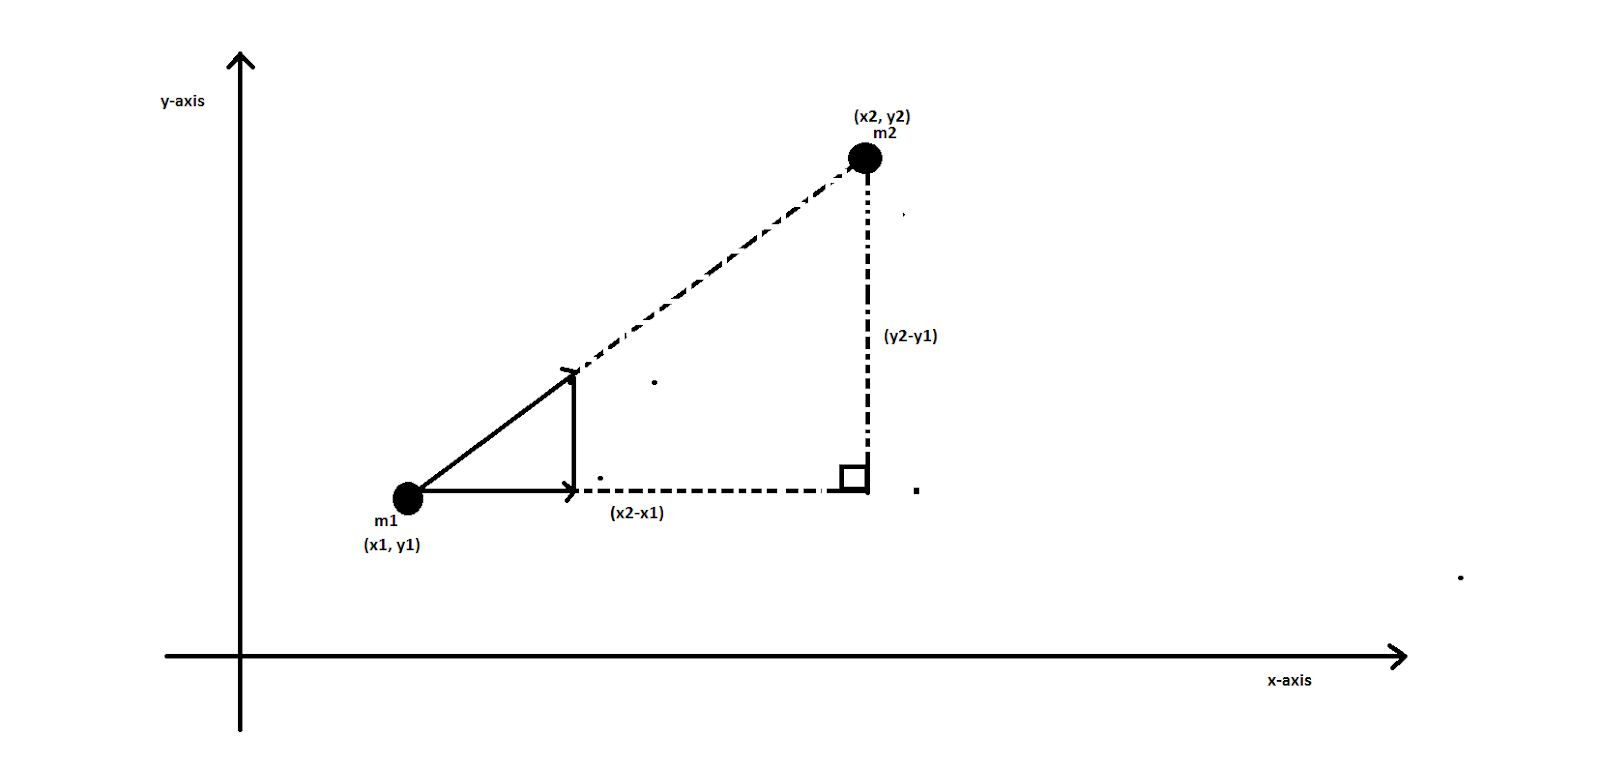
\includegraphics[scale=2.5, width=1\textwidth]{twobody}
	\caption{Two bodies with masses m1 and m2 seperated by a distance r.}
	\label{fig:two-body problem}
\end{figure}
We will now model the two body problem. Let us take a rectangular coordinate frame for the two body problem as shown in the figure above.
\\


The mutual distance apart is r;
\[ r^2 =  (x_2-x_1)^2 + (y_2-y_1)^2  ... \big(1)\]

The magnitude of gravity;
\[ F =  Gm_1m_2 / r^2 ... \big(2)\]
\\
Now the point P1 is attracted to P2 with the force of gravity, F, and can be resolved into the x and y components as;\\
1. along the OX AXIS
\[F_X = Gm_1m_2 / r^2\big(x_2-x_1/r) ... \big(3)\] 
\\
2. along the OY AXIS
\[F_Y = Gm_1m_2 / r^2\big(y_2-y_1/r) ... \big(4)\]
Where, x2-x1/r and y2-y1/r are direct cosines.
\\
For point P2 this will be;\\
1. along the OX AXIS
\[F_X = Gm_1m_2 / r^2\big(x_1-x_2/r) ... \big(5)\] 
\\
2. along the OY AXIS
\[F_Y = Gm_1m_2 / r^2\big(y_1-y_2/r) ... \big(6)\]
Where, x1-x2/r and y1-y2/r are direct cosines.
\\
From Newton’s 2nd Law of motion we have;
\[F=ma\]
\\
We can further work on equations 3) to 6) to obtain the following;\\
1. for particle 1
\[F_X = m_1\big(d^2x/dt^2)= Gm_1m_2 / r^2\big(x_2-x_1/r) ... \big(7)\] 
\[F_Y = m_1\big(d^2y/dt^2)= Gm_1m_2 / r^2\big(y_2-y_1/r) ... \big(8)\]
2. for particle 2
\[F_X = m_2\big(d^2x/dt^2)= Gm_1m_2 / r^2\big(x_1-x_2/r) ... \big(9)\]
\[F_Y = m_2\big(d^2y/dt^2)= Gm_1m_2 / r^2\big(y_1-y_2/r) ... \big(10)\]
\\
Simplifying equations 7) to 10) respectively to obtain equations 11) to 14);\\
1. for particle 1
\[d^2x_1/dt^2= Gm_2 / r^2\big(x_2-x_1/r) ... \big(11)\] 
\[d^2y_1/dt^2= Gm_2 / r^2\big(y_2-y_1/r) ... \big(12)\]
2. for particle 2
\[d^2x_1/dt^2= Gm_1 / r^2\big(x_1-x_2/r) ... \big(13)\]
\[d^2y_1/dt^2= Gm_1 / r^2\big(y_1-y_2/r) ... \big(14)\]
\\
Let us subtract equation 11) from equation 13);
\[\frac{d^2x_2}{dt^2} - \frac{d^2x_1}{dt^2}= \frac{Gm_1} {r^3}\big(\frac{x_1-x_2}{r}) - \frac{Gm_2} {r^3}\big(\frac{x_2-x_1}{r}) ... \big(15)\]

\[\frac{d^2\small(x_2-x_1)}{dt^2}= -\frac{G} {r^3}\bigg[\big(m_1+m_2)-\big(x_2-x_1)\bigg] ... \big(16)\]
Let  \(x = x_2-x_1 ... \big(17)\) and 
\(\mu = G(m1+m2) ... \big(18)\) 
then;
\[\frac{d^2x}{dt^2}+\frac{\mu x}{r^3}=0 ... \big(19)\]
\\
In a similar fashion for equations 12) and 14) we arrive at;
\[\frac{d^2y}{dt^2}+\frac{\mu y}{r^3}=0 ... \big(20)\]
where;
\[y = y_2-y_1 ... \big(21)\]

The solution of this is written as;
\[r = \frac{\frac{h^2}{\mu}}{1+e\cos\theta} ... \big(22)\]

where \(\theta\) is the true anomaly, h is a constant which is twice the rate of description of area by radius vector, e, is the eccentricity of the orbit.\\

To prove this, consider; 
\[r^2 = \big(x_2-x_1)^2+\big(y_2-y_1)^2 ... \big(23)\]
equation 15) and 16) can be combined as; 
\[\frac{d^2r}{dt^2}+\frac{\mu\vec{r}}{r^3}=0 ... \big(24)\]
\[\ddot{\vec{r}}+\frac{\mu\vec{r}}{r^3}=0 ... \big(25)\]
\[\ddot{\vec{r}}=-\frac{\mu\vec{r}}{r^3} ... \big(26)\]\\
crossing both side with \(\vec{r}\) we will have;
\[\vec{r}\times\ddot{\vec{r}}=-\vec{r}\times\frac{\mu\vec{r}}{r^3}\]
\[=0 ... \big(27)\]\\
the left hand side can be written as;
\[\vec{r}\times\ddot{\vec{r}}= \frac{d}{dt}\big(\vec{r}\times\dot{\vec{r}}) ... \big(28)\]\\
since the time derivative of \(\vec{r}\times\dot{\vec{r}}\) is equal to zero, the quantity itself must be a constant, i.e.; \(\vec{r}\times\dot{\vec{r}}=\vec{h}=constant\).\\
The vector \(\vec{h}\) is the angular momentum per unit mass. It is related to the angular momentum vector \(\vec{l}\) by;
\[\vec{l}= m\vec{h}\]
where \(m\) is the mass of the particle.\\

Considering by Kepler's second law, then the motion of this particle over a small time step \(\Delta t\), we have;
\[\Delta A = \frac{1}{2}\arrowvert r\times \dot{r}\Delta t\arrowvert ... \big(29)\]
\[=\frac{1}{2}\arrowvert\vec{h}\arrowvert\Delta t ... \big(30)\]

Therefore;
\[\vec{h}\times\ddot{\vec{r}}=-\frac{\mu\big(\vec{h}\times\vec{r})}{r^3}  ... \big(31)\]
\[=-\frac{\mu}{r^3}\big[\big(\vec{r}\times\dot{\vec{r}})\times\vec{r}  ... \big(32)\]
\[=-\frac{\mu}{r^3}\big[\dot{\vec{r}}\big(\vec{r}\cdot\vec{r})-\vec{r}\big(\vec{r}\cdot\vec{r})]  ... \big(33)\]

now since;
\[\frac{d}{dt}\bigg(\frac{\vec{r}}{r}\bigg)=\frac{1}{r}\dot{r}-\frac{\dot{r}}{r^2}\vec{r}  ... \big(34)\]
\[=\frac{1}{r^3}\big[\dot{\vec{r}}\big(\vec{r}\cdot\vec{r})-\vec{r}\big(\vec{r}\cdot\dot{\vec{r}})]  ... \big(35)\] 

then;
\[\vec{h}\times\dot{r}=-\mu\frac{d}{dt}\bigg(\frac{\vec{r}}{r}\bigg)  ... \big(36)\]

integrating both sides with respect to time will yield;
\[\vec{h}\times\dot{r}= -\mu \frac{\vec{r}}{r}- \vec{A}  ... \big(37)\]

where A is determined by the initial position and velocity.\\

We multiply through by \(\vec{r}\);
\[\big(\vec{h}\times\dot{r})\times\cdot\vec{r}= -\mu \boldmath{r}- \vec{A}\cdot\vec{r}  ... \big(38)\]

If we introduce, \(\nu\), as the true anomaly, the angle between A and the position vector \(\vec{r}\), we obtain;
\[h^2=\mu r + Ar \cos \nu  ... \big(39)\]
since
\[\big(a\times b\big)\cdot c = -\big(c\times b\big)\cdot a  ... \big(40)\]
letting \(P=h^2/\mu \) and \(e = A/\mu \) then;
\[r=\frac{P}{1+e \cos \nu}  ... \big(41)\]
For the above equation for any conic section except a parabola we will have
\[P = a\big(1-e^2)   ... \big(42)\]

therefore;
\[r=\frac{a\big(1-e^2)}{1+e \cos \nu}   ... \big(43)\]

Now we will use this equation to get the position of the satellite in it's orbit from the central body. We still have the problem which is described as; what is the position of a satellite in it's orbit after an elapsed time, \(t-t_o\). We can further refine the problem as; how long does it take for the satellite to move from one point to another in its orbit.

Kepler was able to solve this problem by defining the Mean Anomaly, the part of the orbit form the centre which the satellites sweeps relative to the perigee. Perigee is the shortest point to the centre along the satellite's orbit. 

The change in Mean Anomaly is defined as;
\[M-M_o = n(t-t_o)   ... \big(44)\]

where;
\[n=\sqrt{\frac{\mu}{a^3}}   ... \big(45)\] 

We define a variable \(E\) called the eccentric anomaly which can be written as;
\[cos E = \frac{ae + r \cos \nu}{a}   ... \big(46)\]
\[ \cos E = \frac{e+\cos \nu}{1+e \cos \nu}   ... \big(47)\]

given the above we will have the mean anomaly as;
\[M= E-sinE   ... \big(48)\]
this is Kepler's equation.

